% !!!IMPORTANT NOTE: Please read carefully all information including those preceded by % sign
%Before you compile the tex file please download the class file AIMS.cls from the following URL link to the
%local folder where your tex file resides. http://aimsciences.org/journals/tex-sample/AIMS.cls.
\documentclass{aims}
\usepackage{amsmath}
  \usepackage{paralist}
  \usepackage{graphics} %% add this and next lines if pictures should be in esp format
  \usepackage{epsfig} %For pictures: screened artwork should be set up with an 85 or 100 line screen
\usepackage{graphicx}  \usepackage{epstopdf}%This is to transfer .eps figure to .pdf figure; please compile your paper using PDFLeTex or PDFTeXify.
 \usepackage[colorlinks=true]{hyperref}
   % Warning: when you first run your tex file, some errors might occur,
   % please just press enter key to end the compilation process, then it will be fine if you run your tex file again.
   % Note that it is highly recommended by AIMS to use this package.
\hypersetup{urlcolor=blue, citecolor=red}
%\usepackage{hyperref}

\usepackage[utf8]{inputenc}

  \textheight=8.2 true in
   \textwidth=5.0 true in
    \topmargin 30pt
     \setcounter{page}{1}

% The next 5 line will be entered by an editorial staff.
\def\currentvolume{X}
 \def\currentissue{X}
  \def\currentyear{200X}
   \def\currentmonth{XX}
    \def\ppages{X--XX}
     \def\DOI{10.3934/xx.xx.xx.xx}

 % Please minimize the usage of "newtheorem", "newcommand", and use
 % equation numbers only situation when they provide essential convenience
 % Try to avoid defining your own macros

\newtheorem{theorem}{Theorem}[section]
\newtheorem{corollary}{Corollary}
\newtheorem*{main}{Main Theorem}
\newtheorem{lemma}[theorem]{Lemma}
\newtheorem{proposition}{Proposition}
\newtheorem{conjecture}{Conjecture}
\newtheorem*{problem}{Problem}
\theoremstyle{definition}
\newtheorem{definition}[theorem]{Definition}
\newtheorem{remark}{Remark}
\newtheorem*{notation}{Notation}
\newcommand{\ep}{\varepsilon}
\newcommand{\eps}[1]{{#1}_{\varepsilon}}


%% Place the running title of the paper with 40 letters or less in []
 %% and the full title of the paper in { }.
\title[Globalizer: a supercomputer software] %Use the shortened version of the full title
      {Globalizer: a novel supercomputer software system for solving time-consuming global optimization problems}

% Place all authors' names in [ ] shown as running head, Leave { } empty
% Please use `and' to connect the last two names if applicable
% Use FirstNameInitial.  MiddleNameInitial. LastName, or only last names of authors if there are too many authors
\author[V. P. Gergel, K. A. Barkalov and A. V. Sysoyev]{}

% It is required to enter 2010 MSC.
\subjclass{Primary: 90C26; Secondary: 65Y05.}
% Please provide minimum  5 keywords.
 \keywords{Global optimization, information-statistical theory, parallel computing, high-performance
computer systems,  supercomputer technologies.}

% Email address of each of all authors is required.
% You may list email addresses of all other authors, separately.
 \email{victor.gergel@itmm.unn.ru}
 \email{konstantin.barkalov@itmm.unn.ru}
 \email{alexander.sysoyev@itmm.unn.ru}

% Put your short thanks below. For long thanks/acknowlegements,
%please go to the last acknowlegments section.
\thanks{The study was supported by the Russian Science Foundation, project No 16-11-10150.}

% Add corresponding author at the footnote of the first page if it is necessary.
% Plase add $^*$ adjacent to the corresponding author's name on the first page.
% The example shown in this template is if the first author is the corresponding author.
\thanks{$^*$ Corresponding author: Konstantin  Barkalov}

\begin{document}
\maketitle

% Enter the first author's name and address:

\centerline{\scshape Victor Gergel, Konstantin  Barkalov$^*$ and Alexander Sysoyev}
\medskip
{\footnotesize
 % please put the address of the second  and third author
 \centerline{Lobachevsky State University of Nizhny Novgorod}
   \centerline{23, Gagarin Avenue}
   \centerline{Nizhny Novgorod, Russia}
}

\bigskip

% The name of the associate editor will be entered by an editorial staff
% "Communicated by the associate editor name" is not needed for special issue.
 \centerline{(Communicated by the associate editor name)}


%The abstract of your paper
\begin{abstract}
In this paper, we describe the Globalizer software system for solving the global
optimization problems. The system is designed to maximize the use of computational
potential of the modern high-performance computational systems in order to solve the
most time-consuming optimization problems. The highly parallel computations are facilitated
using various distinctive computational schemes: processing several optimization
iterations simultaneously, reducing multidimensional optimization problems using multiple
Peano space-filling curves, and multi-stage computing based on the nested block reduction schemes.
These novelties provide for the use of the supercomputer system capabilities with shared
and distributed memory and with large numbers of processors to solve the global
optimization problems efficiently.
\end{abstract}

%The title of your section 1
\section{Introduction}\label{sec:intro}

Global (or multiextremal) optimization problems are among the most complex problems
in both theory and practice of optimal decision making. In these kinds of problems,
the criterion to be optimized has several local optima within the search domain,
which have different values. The existence of several local optima essentially makes
finding the global optimum difficult essentially, since it requires examining the whole feasible
search domain. The volume of computations for solving global optimization problems
can increase exponentially with increasing number of varied parameters.
\par
These global optimization problem features impose special requirements on the quality
of the optimization methods and on the software to implement these ones. The global
optimization methods should be highly efficient, and the software systems should be developed on
a good professional basis. In general, the global optimization problems can be solved at
a reasonable time by employing parallel computations on modern supercomputer systems only.
\par
The general state of the art in the field of global optimization has been presented in a
number of key monographs  \cite{floudasPardGO}, \cite{horstTuyGO}, \cite{locatelliSchoenGO}, \cite{pinterGO}, \cite{strSergGO}, \cite{zilinskTornGO}, \cite{zhigljavskyRandGO}, etc.
The development of optimization methods, which use the high-performance computational
systems to solve the time-consuming global optimization problems, is an area of
intensive research --- see, for instance, \cite{censorZeniosParGO}, \cite{ciegisHentyParGO},
\cite{luqueAlbaGA}, \cite{stronginGergelBarkalovParGO}, \cite{strSergGO}. The obtained
theoretical results provide the efficient solutions of many applied global
optimization problems in various fields of scientific and technical applications \cite{Famularo1999}, \cite{fasanoPinter2013},
\cite{floudasPardalosGOState}, \cite{Kvasov2015}, \cite{Menniti}, \cite{locatelliSchoenGO},
\cite{luqueAlbaGA}, \cite{pardalosZhigljavskyZilinskas2016}, \cite{pinterGO}.
\par
At the same time, the practical implementation of these global optimization algorithms
within the framework of industrial software systems is quite limited. In many cases,
software implementations are experimental in nature and are used by the developers
themselves to obtain the results from the computational experiments required for the
scientific publications. This situation originates from high development costs of the
professional software systems, which can be used by numerous users. In addition, the global
optimization problems could be solved in an automatic mode rarely because of the
complexity of these ones. The user should actively control the global search
process that implies an adequate level of qualification in the field of optimization
(particularly, the user should know and understand the global optimization methods well).
\par
In the market of the global optimization software, one can select from the following systems:
\begin{itemize}
\item LGO (Lipschitz Global Optimization) \cite{pinterGO} was designed to solve the global
optimization problems, where the criteria and constraints satisfy the Lipschitz condition.
The system is a commercial product based on the diagonal extensions of the one-dimensional multiextremal optimization algorithms.
\item GlobSol \cite{kearfott2009} is oriented on solving the global optimization
problems as well as of the systems of the nonlinear equations. The system includes
the interval methods based on the branch and bound approach. There are some extensions
of the system for the parallel computations, and it is available for free usage.
\item LINDO \cite{linSchrage2009} is featured by a wide spectrum of optimization methods for solving linear, integer, stochastic, nonlinear, and global optimization problems. The ability to interact with the Microsoft Excel software environment is a useful feature of this system. The system is widely used in the practical applications and is available for free usage.
\item IOSO (Indirect Optimization on the basis of Self-Organization) \cite{iosoDescription} is oriented on solving a wide class of the optimization problems including the global optimization ones. The system is widely used to solve the applied problems in various application fields. There is a version of the system for exciting on the parallel computational systems. The system is a commercial product, but it is available for the trial usage.
\item MATLAB Global Optimization Toolkit \cite{venkataraman2009} contains a wide
spectrum of methods for solving the global optimization problems, including multistart
algorithms, global pattern search, simulated annealing methods, etc. The library is
compatible with the TOMLAB system \cite{holmstromEdvall2004}, which is an additional
MATLAB extension. It should also be noted that similar libraries for solving the global
optimization problems are available for MathCAD, Mathematica, and Maple systems as well.
\item BARON (Branch-And-Reduce Optimization Navigator) \cite{sahinidis1996} was designed to
solve continuous integer programming and global optimization problems using the branch and
bound approach. BARON is included in the GAMS (General Algebraic Modeling System) system \cite{bussieckMeeraus2004}.
\item Global Optimization Library in R is a large collection of optimization methods
implemented in the R language \cite{mullen2014}. Among these methods, stochastic and
deterministic global optimization algorithms and the branch and bound method were implemeted.
\end{itemize}
\par
The list provided above is certainly not exhaustive – additional information on the
software systems for solving a wider spectrum of optimization problems can be found, for example, in
\cite{mongeauKarsentyRouze2000}, \cite{pinter2009}, \cite{riosSahinidis2013}.
\par
In this paper, a novel Globalizer software system is presented. Globalizer expands the collection of the parallel optimization systems mentioned above. The Globalizer system was designed to solve the time-consuming multiextremal optimization problems that is an advantage of the system. In order to obtain the global optimized solutions within a reasonable time, the system exploits the huge computational potential of high-performance massively parallel systems.

The further structure of the paper is as follows. In Section \ref{sec:problem},
a statement of the multidimensional global optimization problem is given and an
approach for reducing this one to a one-dimensional optimization problem is described.
In Section \ref{sec:parallel}, the parallel computation schemes are discussed and
the parallel optimization methods are presented. In Section \ref{sec:arch}, the architecture of
the Globalizer system is described. In Section \ref{sec:experiments}, the results of the numerical experiments,
which confirm the parallel efficiency of the Globalizer system, are presented. Finally,
Section \ref{sec:concl} presents the conclusions and some ideas for the future research.

\section{Multidimensional Global Optimization Problems and Dimension Reduction}
\label{sec:problem}
In this paper, the core class\footnote{In general, the Globalizer can be applied for solving
multicriterial multiextremal multidimensional optimization problems with nonlinear constraints.}
of optimization problems, which can be solved using
Globalizer, is formulated. This class involves the multidimensional global
optimization problems without constraints, which can be defined in the following way:
\begin{equation}
\label{eq:task}
\begin{array}{cr}\\
  \varphi(y^*)=\min\{\varphi(y):y\in D\} \\
  D=\{y\in \mathbf{R}^N:a_i\leq y_i\leq{b_i}, 1\leq{i}\leq{N}\}
\end{array}
\end{equation}
It is supposed, that the objective function \(\varphi(y)\) satisfies the Lipschitz condition
\begin{equation}
\label{eq:lip}
|\varphi(y_1)-\varphi(y_2)|\leq L\Vert y_1-y_2\Vert,y_1,y_2\in D,
\end{equation}
where \(L>0\) is the Lipschitz constant, and \(||\cdot||\) denotes the norm in \(\mathbf{R}^N\) space.
\par
Usually, the minimized function \(\varphi(y)\) is defined as a computational procedure,
according to which the value \(\varphi(y)\) can be calculated for any vector \(y\in D\)
(let us further call such a calculation \textit{a trial}). It is supposed that this procedure
is a time-consuming one. As a result, the overall time of solving the optimization
problem (\ref{eq:task}) is determined, first of all by the number of executed trials.
It should also be noted that the requirement of the Lipschitz condition (\ref{eq:lip})
is highly important, since an estimate of the global minimum can be constructed on the
base a finite number of computed values of the optimized function only in this case .
\par
As it has been shown earlier by many researchers
(see, for instance, [12], [25], [38], [51]),
finding the numerical estimate of the global optimum implies constructing a coverage of
the search domain \(D\). As a result, the computational costs of solving the global
optimization problems are readily very high even for a small number of varied parameters
(the dimensionality of the problem). A notable reduction in the volume of computations
can be achieved when the coverage of the search domain is non-uniform, i. e. the series
of trial points is only dense in a vicinity of the global optimum point. The construction
of such a non-uniform coverage could be provided in an adaptive way, when the selection
of the next trial points is determined by using the search information ((the preceding
trial points and the values of the minimized function at these points) obtained in the course
of computations. This necessary condition complicates considerably the computational schemes
for global optimization methods since it implies a complex analysis of a large amount
of multidimensional search information. As a result, many optimization algorithms use
various approaches to the dimensional reduction [38], [46], [48], [50], [51].
\par
Within the framework of the information-statistical global optimization theory,
the Peano space-filling curves (or evolvents) \(y(x)\) mapping the interval \([0,1]\)
onto an \(N\)-dimensional hypercube \(D\) unambiguously are used for the dimensionality
reduction [46], [48], [50], [51].
\par
As a result of the reduction, the initial multidimensional global optimization
problem (\ref{eq:task}) is reduced to the following one-dimensional problem:
\begin{equation}
\label{eq:oneDimTask}
\varphi(y(x^*))=\min\{\varphi(y(x)):x\in [0,1]\}
\end{equation}
\par
It is important to note that this dimensionality reduction scheme transforms the minimized
Lipschitzian function from (\ref{eq:task}) to the corresponding one-dimensional
function \(\varphi(y(x))\), which satisfy the uniform H{\"o}lder condition i. e.
\begin{equation}
\label{eq:holder}
|\varphi(y(x_1))-\varphi(y(x_2))|\leq H{|x_1-x_2|}^{\frac{1}{N}},x_1,x_2\in[0,1]
\end{equation}
where the constant H is defined by the relation \(H=4L\sqrt{N}\), \(L\) is the Lipschitz
constant from (\ref{eq:lip}), and \(N\) is the dimensionality of the optimization problem (\ref{eq:task}).
\par
The algorithms for the numerical construction of the Peano curve approximations are
presented in \cite{strSergGO}. As an illustration, an approximation of the Peano curve
for the third density level is shown in Figure \ref{fig:peanoC}. Figure \ref{fig:peanoC}
demonstrates the movement order in a two-dimensional domain to construct the Peano
curve approximation; the precision of the Peano curve approximation is determined by the
density level used in the construction.
\begin{figure}
    \centering
    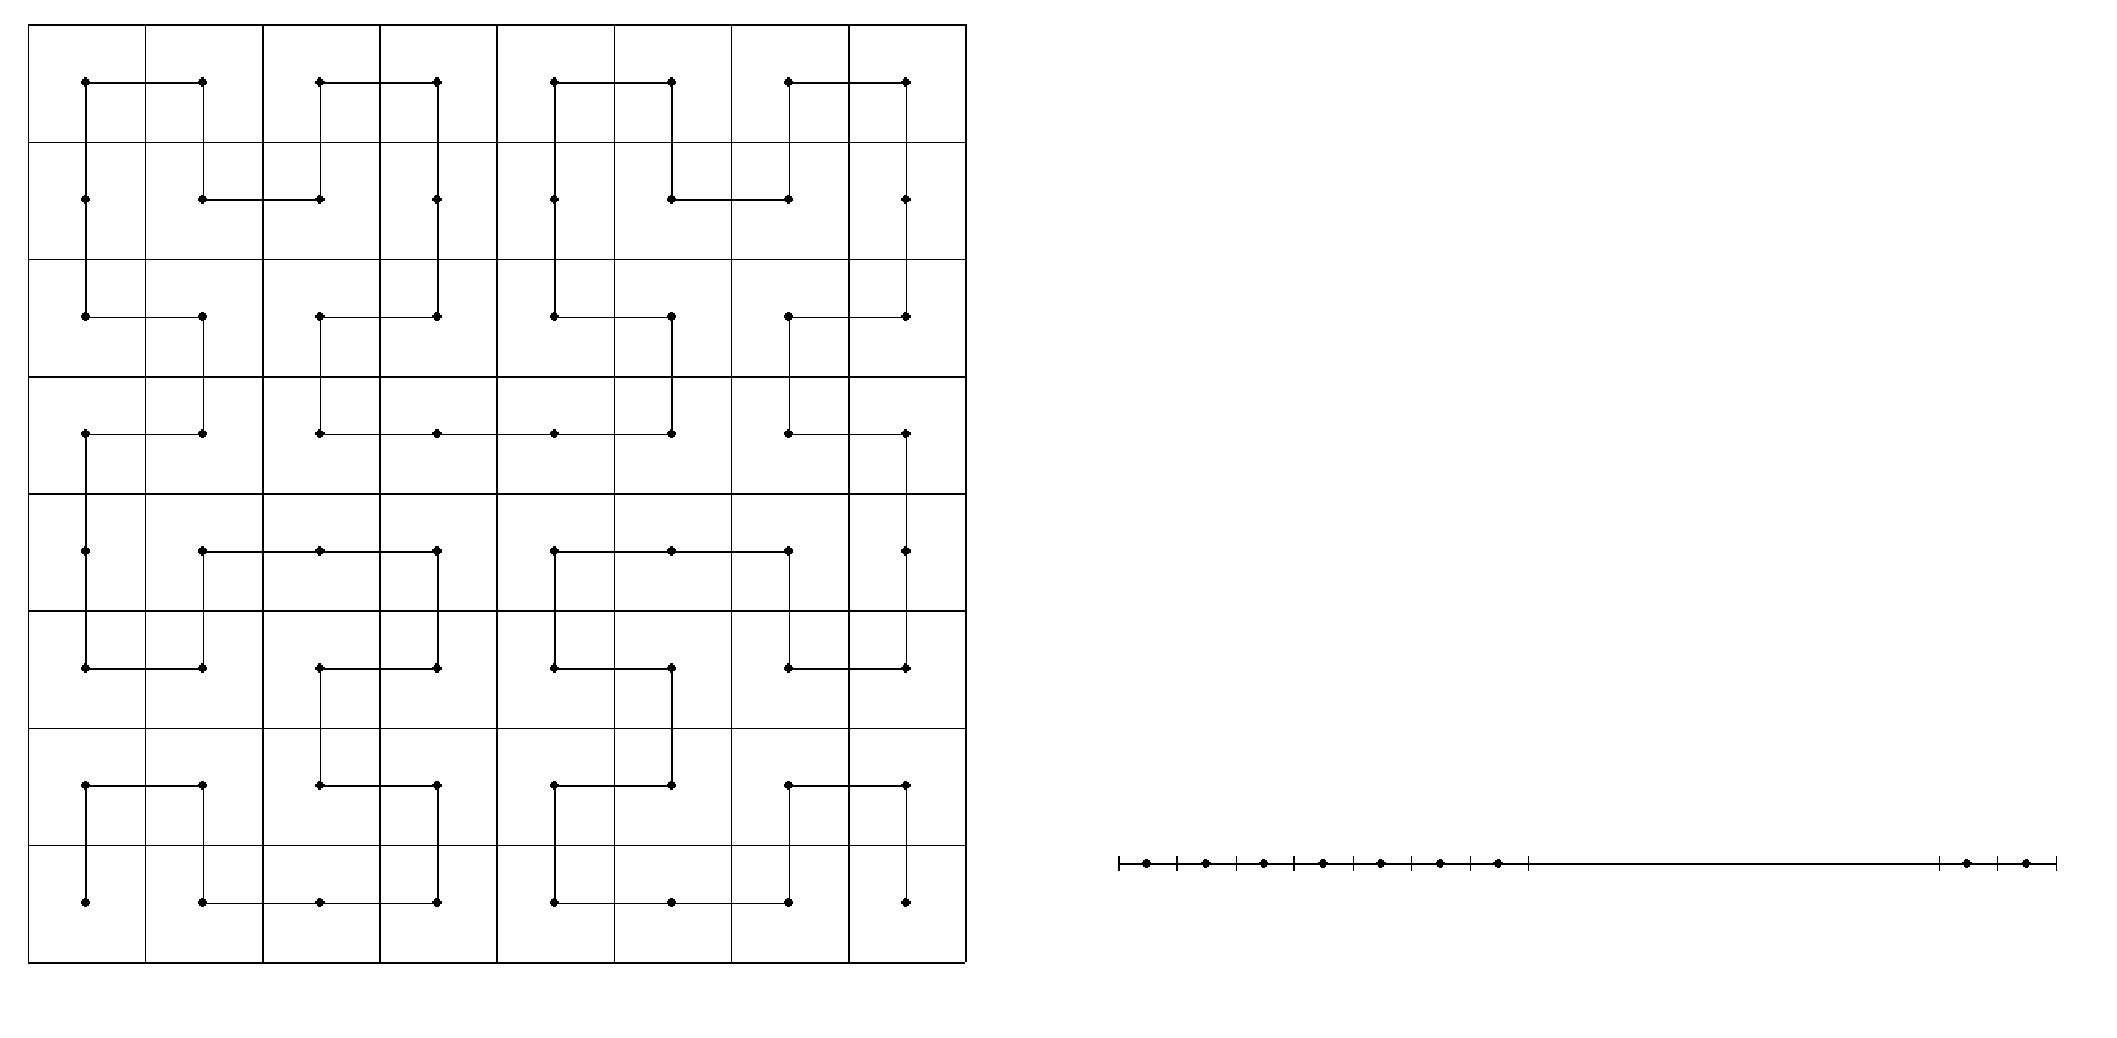
\includegraphics[width=0.85\textwidth]{pictures/peanoC.eps}
    \caption{A Peano curve approximation for the third level}
    \label{fig:peanoC}
\end{figure}

\par
The computational scheme obtained as a result of the dimensionality reduction consists of the following
(see Figure \ref{fig:peanoCUsage}):
\begin{itemize}
  \item The optimization algorithm performs the minimization of the reduced one-dimensional
  function \(\varphi(y(x))\) from (\ref{eq:oneDimTask}),
  \item After determining the next trial point \(x\), a multidimensional image \(y\) in the mapping \(y(x)\) is calculated,
  \item The value of the initial multidimensional function \(\varphi(y)\) is calculated at the multidimensional point \(y\in D\),
  \item The calculated value \(z=\varphi(y)\) is used further as the value of the reduced one-dimensional function \(\varphi(y(x))\) at the point \(x\).
\end{itemize}

\begin{figure}
    \centering
    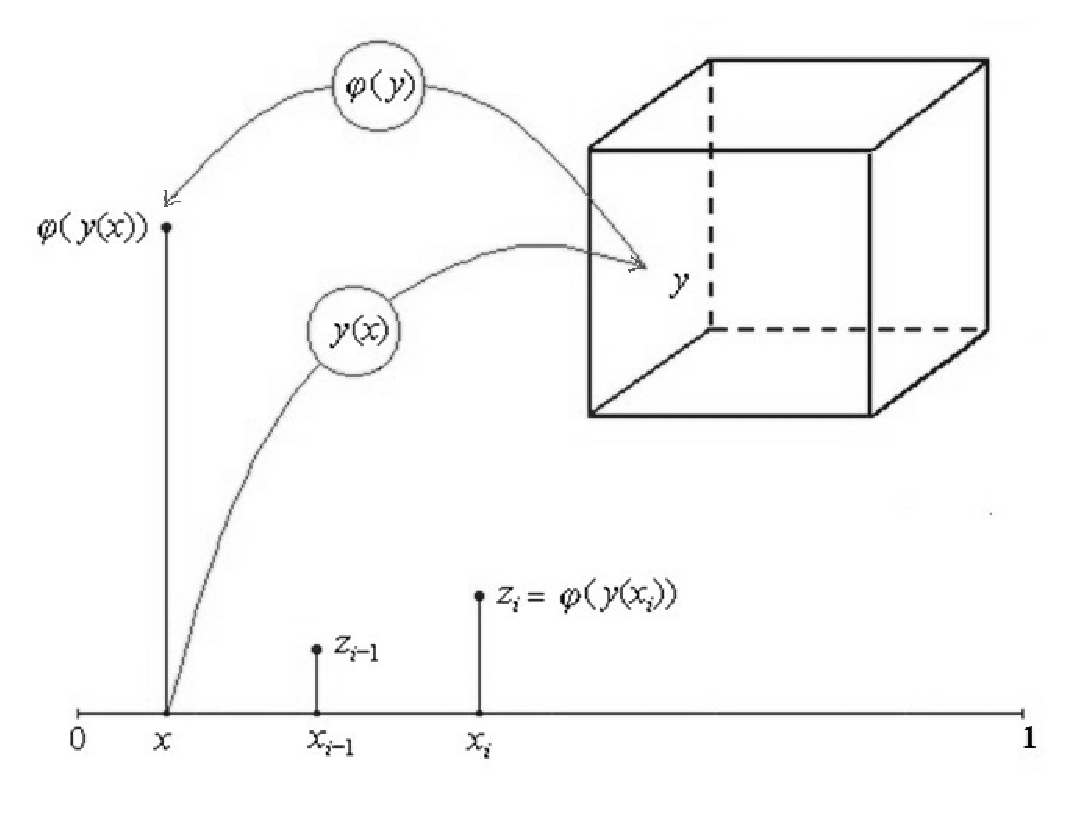
\includegraphics[width=0.55\textwidth]{pictures/peanoCUsage.eps}
    \caption{The computational scheme for obtaining the value of the reduced one-dimensional function \(\varphi(y(x))\)}
    \label{fig:peanoCUsage}
\end{figure}

\section{Parallel Computations for Solving Global Optimization Problems}
\label{sec:parallel}
Let us consider the parallelization methods used widely in the theoretical and
practical application of parallel computing within the context of global optimization problems:
\begin{itemize}
  \item The distribution of the search domain \(D\) among the available computing units
  (data parallelization scheme). In the case of optimization problems, this approach is
  insufficient, since in organizing such computations the subdomain, which contain the
  sought global minimum, will be processed by only one processor, and, therefore,
  all of the remaining processors would perform the excess computations.
  \item The parallelization of the computational schemes for optimization algorithms
  (task parallelization scheme). This approach is also insufficient since the direct
  computational costs for executing optimization algorithms are relatively low
  (the majority of computations in the course of a global search are represented by
  calculations of the optimized function values due to the initial assumption of
  considerable computational costs for such calculations).
  \item The parallelization of the computations executed in order to obtain values
  for the optimized function. This approach can be applied since the most computationally
  costly part of the global search process will be parallelized. However, this method is not
  featured by the generality (the development of parallelization methods is to be performed
  every time from scratch while solving each particular optimization problem).
\end{itemize}
\par
Within the framework of information-statistical theory, a general approach to
parallelization computations when solving global optimization problems has been
proposed --- \textit{the parallelism of computations is provided by means of simultaneously
computing the values of the minimized function \(\varphi(y)\) at several different
points within the search domain \(D\)} – see, for example, \cite{stronginGergelBarkalovParGO}, \cite{strSergGO}.
This approach provides parallelizaion for the most costly part of computations in the global search process.
\par
The global optimization algorithms implemented in Globalizer will be described step-by-step below.
In Subsection \ref{subsec:corepar}, the core sequential multidimensional algorithm of global search (MAGS) will be presented.
In Subsection \ref{subsec:sharedpar}, a parallel generalization of the MAGS algorithm for parallel computations on
computer systems with shared memory will be described. In Subsection \ref{subsec:distribpar}, the scheme
for parallel computations by multiprocessor systems with distributed memory will be provided.

\subsection{Core Multidimensional Generalized Algorithm of Global Search}
\label{subsec:corepar}
The information-statistical theory of global search formulated in \cite{strongin1978}, \cite{strSergGO}
has served as a basis for the development of a large number of efficient multiextremal optimization methods --- see, for example, \cite{barkalovGergel2014}, \cite{Pizzuti}, \cite{gergel1996}, \cite{gergel1997}, \cite{grishaginStrongin1984}, \cite{sergeyev1995}, \cite{sergeyev1999}, \cite{sergeyevGrishagin1994}, \cite{sergeyevGrishagin2001}, \cite{sergeyevStronginLera2013}, \cite{Famularo2001} etc.
\par
Multidimensional Algorithm of Global Search (MAGS) established the basis for the
methods applied in Globalizer. The general computational scheme of MAGS can be
presented as follows --- see \cite{strongin1978}, \cite{strSergGO}.
\par
Let us introduce a simpler notation for the problem being solved on a computing node
\begin{equation}
\label{eq:oneDimFunc}
f(x) = \varphi(y(x)):x\in [0,1].
\end{equation}
\par
The initial iteration of the algorithm is performed at an arbitrary point \(x^1(0,1)\).
Let us assume further \(k\), \(k>1\), iterations of a global search are to be completed.
The selection of the trial point \(k+1\) for the next iteration is performed according to the following rules.
\par
\textit{Rule 1}. To renumber the points for the preceding trials by the lower indices in order of increasing value of coordinates
\begin{equation}
  \label{step1}
0=x_0<x_1<...<x_{k+1}=1.
\end{equation}
The points \(x_0\), \(x_k\) were introduced additionally for convenience in further explanation,
the values of the minimized function \(z_0\), \(z_k\) at these points are undefined.
\par
\textit{Rule 2}. To compute a current estimate of the H{\"o}lder constant \(H\) from (\ref{eq:holder})
\begin{equation} \label{step2}
m=\max_{1\leq i\leq k}\frac{|z_i-z_{i-1}|}{\rho_i}, \;
M = \left\{
   \begin{array}{lr}
     rm, & m > 0,\\
     1, & m = 0,
   \end{array}
  \right.
\end{equation}
as the maximum of the relative differences of the minimized function \(f(x)\) from (\ref{eq:oneDimFunc})
on the set of executed trial points \(x_i,1\leq i\leq k\) from (\ref{step1}). Further, \(\rho_i=(x_i-x_{i-1})^\frac{1}{N},1\leq i\leq k+1\).
The constant \(r\), \(r>1\), is the \textit{parameter} for the algorithm.
\par
\textit{Rule 3}. For each interval \((x_{i-1},x_i),1\leq i\leq k+1\), compute the characteristics \(R(i)\) where
\[
R(i)=2\rho_i-4\frac{z_i}{M},\quad i=1,
\]
\begin{equation} \label{step3}
R(i)=\rho_i+\frac{(z_i-z_{i-1})^2}{M^2\rho_i}-2\frac{z_i+z_{i-1}}{M},\quad 1<i<k+1, \\
\end{equation}
\[
R(i)=2\rho_{i}-4\frac{z_{i-1}}{M},\quad i=k+1.
\]

\par
\textit{Rule 4}. To determine the interval with the maximum characteristic
\begin{equation} \label{step4}
R(t)=\max_{1\leq i \leq k+1}R(i).
\end{equation}
\par
\textit{Rule 5}. To execute a new trial (computation of the minimized function value \(f(x)\))
at the point \(x^{k+1}\) located within the interval with the maximum characteristic from (\ref{step4})
\begin{equation} \label{step5}
  x_{k+1}=\frac{x_t+x_{t-1}}{2}-\mathrm{sign}(z_{t}-z_{t-1})\frac{1}{2r}\left[\frac{|z_{t}-z_{t-1}|}{M}\right]^N,\; \textrm{ if } 1<t<k+1,
\end{equation}
\[
  x_{k+1}=\frac{x_t+x_{t-1}}{2},\; \textrm{ if } t=1 \textrm{ or } t=k+1.
\]

\par
The stop condition by which the trials are terminated, is defined by the inequality
\begin{equation}
  \label{eq:stop_1}
\rho_t<\varepsilon
\end{equation}
for the interval with the maximum characteristic from (\ref{step4}) and \(\varepsilon >0\) is the predefined
accuracy of the problem solution. If the stop condition is not satisfied, the index \(k\) is incremented by unity,
and a new global search iteration is executed.
\par
In order to explain the algorithm presented above, let us note the following.
The characteristics \(R(i), 1\leq i\leq k+1\), calculated according to (\ref{step3})
could be interpreted as some measures of importance to the intervals with respect to
location of the global minimum point. Thus, the scheme for selecting the interval
for executing the next trial described in (\ref{step4}), (\ref{step5}) becomes more clear --- the point of every next
global search iteration is selected within the interval where the global minimum point can most likely be found.
\par
The conditions for the algorithm’s convergence described above were examined, for example, in \cite{strSergGO}.

\subsection{Parallel Computations for Systems with Shared Memory}
\label{subsec:sharedpar}
Modern supercomputer computational systems consist of plenty of computer nodes,
which include several multicore processors. At that, random access memory is
shared for the computing nodes --- the content of any memory element can be read (written)
by any computer cores available at any arbitrary moment. In most cases, shared memory is
uniform --- the time characteristics for accessing memory are the same for all computer
cores and for all memory elements.
\par
The following speculations can form the basis for selecting parallel computation
organization methods. As was mentioned above when describing the MAGS algorithm,
the characteristics \(R(i),1\leq i\leq k+1\), calculated according to (\ref{step3})
can be interpreted as some measures of the importance of intervals with respect to the location of
the global minimum point. Following this understanding, each successive global search
iteration is executed within the most important interval with the maximum value of the
characteristic. So far, in this case it is obvious how to select the other intervals for
organizing simultaneous computations of the minimized function values at several different
points within the search domain as well --- these should be the intervals with the next
magnitudes of characteristics.
\par
The computational scheme of the Parallel Multidimensional Algorithm of Global Search for
computer systems with shared memory (PMAGS) was developed based the approach considered
above and is practically identical to the MAGS scheme --- the differences consist just in the
following set of rules --- see \cite{strSergGO}, \cite{stronginGergelBarkalovParGO}.
\par
\textit{Rule 4'}. To arrange the characteristics of the intervals obtained according to (\ref{step3}) in decreasing order
\begin{equation}
\label{step4par}
R(t_1)\geq R(t_2)\geq \dots \geq R(t_{k})\geq R(t_{k+1})
\end{equation}
and to select \(p\) intervals with the indices \(t_j,1\leq j\leq p\), with
the highest values of characteristics (\(p\) is the number of processors/cores used for the parallel computations).
\par
\textit{Rule 5'}. To execute new trials (computations of values for the minimized
function \(f(x)\)) at the points \(x_{k+j},1\leq j\leq p\), located in the
intervals with the highest characteristics from (\ref{step4par})

\begin{equation} \label{step5par}
x_{k+j}=\frac{x_{t_j}+x_{t_j-1}}{2}-\mathrm{sign}(z_{t_j}-z_{t_j-1})\frac{1}{2r}\left[\frac{|z_{t_j}-z_{t_j-1}|}{M}\right]^N,\; \textrm{ if } 1<t_j<k+1,
\end{equation}
\[
x_{k+j}=\frac{x_{t_j}+x_{t_j-1}}{2},\; \textrm{ if } t_j=1 \textrm{ or } t_j=k+1.
\]
\par
The stop condition for the algorithm (\ref{eq:stop}) should be checked for all
intervals from (\ref{step4par}), in which the scheduled trials are executed
\begin{equation}
  \label{eq:stop}
\rho_{t_j}<\varepsilon,1\leq j\leq p.
\end{equation}
As before, if the stop condition is not fulfilled, the index \(k\) is
incremented by \(p\), and a new global search iteration is executed.
\par
The conditions for the developed parallel algorithm’s convergence and for the
non-redundancy of parallel computations have been examined in \cite{strSergGO}.
Thus, in particular, when the conditions for convergence are satisfied, the parallel
computations are non-redundant as compared to the sequential method when using up to
\(2^N\) processors/cores (where \(N\) is the dimensionality of the global optimization problem being solved).

\subsection{Parallel Computations for Systems with Distributed Memory}
\label{subsec:distribpar}
The next level of parallel computations in high-performance computer systems consists of
using several computational nodes. For that, each computational node has its own separate
memory and, in this case, the interaction between different nodes can be provided by
means of data transfer only via the computer communication network.
\par
To organize parallel computations for multiprocessor systems with distributed memory, using a set of mappings
\begin{equation}
  \label{eq:maps}
Y_s(x)=\{y^1(x),\dots,y^s(x)\}
\end{equation}
instead of applying a single Peano curve \(y(x)\) has been proposed in \cite{strongin1992}, \cite{strSergGO}.
In order to build the set \(Y_s(x)\), several different approaches can be applied.
Thus, for example, in \cite{strongin1992} a scheme has been applied by which each
mapping \(y_i(x)\) from \(Y_s(x)\) is built as the result of some shift along the main
diagonal of the hypercube \(D\). This way, the set of constructed Peano curves enables the
close prototypes \(x'\), \(x''\)  to be obtained from the interval \([0,1]\) for any close
multidimensional images \(y'\), \(y''\) from \(D\) differing in one coordinate,
only for some mapping \(y_k(x), 1\leq k\leq s\).
\par
Some other methods for constructing multiple mappings have been examined in \cite{stronginGergelBarkalovParGO}.
\par
The set of mappings \(Y_s(x)\) from (\ref{eq:maps}), for multidimensional problem (\ref{eq:task})
generates \(s\) subsidiary information-linked one-dimensional problems of the kind (\ref{eq:oneDimTask}):
\begin{equation}
  \label{eq:oneDimProblemSerie}
  \varphi(y^l(x^*))=\min\{\varphi(y^l(x)):x\in [0,1]\},1\leq l\leq s.
\end{equation}
\par
It is important to note that the family of one-dimensional problems
\[
\varphi(y^l(x)),1 \leq l \leq s,
\]
obtained as a result of the dimensional reduction is information-linked --- the function
values computed for any problem \(\varphi(y^l(x))\) from the family (\ref{eq:oneDimProblemSerie}) can be used for all
of the remaining problems of this family.
\par
The information compatibility of the problems from the family (\ref{eq:oneDimProblemSerie}) allows the parallel
computations to be organized in an obvious enough way. Thus, each particular problem can
be solved by a separate processor in the computing system; the exchange of search information
between the processors should be performed during the course of the computations.
As a result of using such a parallelization method, a unified approach for organizing parallel
computations for a multiprocessor computer systems with distributed, as well as shared
memory can be developed. This method consists of the following.
\begin{enumerate}
  \item The family of reduced one-dimensional information-linked problems (\ref{eq:oneDimProblemSerie}) is
  distributed among the computational nodes of a multiprocessor system. One problem,
  as well as several others from within the family, can be allocated to each particular computational node.
  \item The Parallel Multidimensional Algorithm of Global Search (PMAGS, see Subsection \ref{subsec:sharedpar})
  is applied to solve the allocated problems from the family (\ref{eq:oneDimProblemSerie})
  at each computational node, supplemented by the following rules of information interaction.
  \begin{enumerate}
    \item Prior to beginning a new trial at any point \(x'\in [0,1]\) for any problem \(\varphi(y_l(x)),1\leq l\leq s\),
    the following should be performed:
    \begin{itemize}
      \item compute the image \(y'\in D\) for the point \(x'\in [0, 1]\) according to the mapping \(y_l(x)\),
      \item determine  the prototypes \(x_i',1\leq i\leq s\), for each
      problem from the family (\ref{eq:oneDimProblemSerie}),
      \item send the prototypes \(x_i',1\leq i\leq s\) to all computational
      nodes employed in order to exclude the repeated selection of the intervals in
      which the prototypes fall, for using them to determine the points for new trials.
      To organize the data transfer, a queue can be formed at each computational
      node for sending the trial points and receiving the minimized function values at these points.
    \end{itemize}
    \item After completing any trial for any problem \(\varphi(y_l(x)),1\leq l\leq s\), at any point
    \(x'\in[0,1]\), it is necessary:
    \begin{itemize}
      \item to determine all prototypes \(x_i',1\leq i\leq s\), for the point of the completed trial
      for each problem from the family (\ref{eq:oneDimProblemSerie}),
      \item to send the prototypes \(x_i',1\leq i\leq s\), and the result of the
      trial \(z'=\varphi(y_l(x'))\) to all computational nodes employed to include the
      obtained data into the search information processed within the rules of the parallel global search algorithm.
    \end{itemize}
    \item Prior to starting the next global search iteration, the algorithm should
    check the queue of the received data; if there are some data in the queue,
    they should be included in the search information.
\end{enumerate}
\end{enumerate}
\par
The possibility of asynchronous data transfer (the computational nodes process received
data only upon receipt) is a meaningful feature of such a scheme for organizing parallel computations.
\par
In addition, there is no single managing node within this scheme. The number of
computational nodes can vary during the course of the global search, and excluding any
node does not result in the loss of the sought global minimum of the minimized multiextremal function.
\par
This computational scheme generates the Generalized Parallel Multidimensional Algorithm of
Global Search (GPMAGS) for high-performance computing systems, which may include many
multiprocessor (multicore) computational nodes with distributed memory as well as
accelerators for computations based on Intel Xeon Phi processors and on general purpose graphic processors.
\par
Additional information on organizing such parallel computation schemes is provided in \cite{gergelSidorov2015}.


\section{Globalizer System Architecture}
\label{sec:arch}
As previously mentioned in Section \ref{sec:intro}, the development of software systems
for global optimization is complex professional work. The optimization systems should
include advanced optimization methods, provide for the accumulation and efficient
processing of search information, include various forms of visualization for the results,
provide tools for interacting with users, etc. All the features pointed out above
become much more complicated when organizing parallel computations using high-performance
multiprocessor systems of varying architectures.
\par
The Globalizer considered in this paper expands the family of global optimization
software systems successively developed by the authors during the past several years.
One of the first developments was the SYMOP multiextremal optimization system \cite{gergel1993},
which has been successfully applied for solving many optimization problems. A special
place is occupied by the ExaMin system (see, for example, \cite{barkalovGergel2015}),
which was developed and used extensively to investigate the application of novel parallel
algorithms to solve global optimization problems using high-performance multiprocessor computing systems.

\begin{figure}
    \centering
    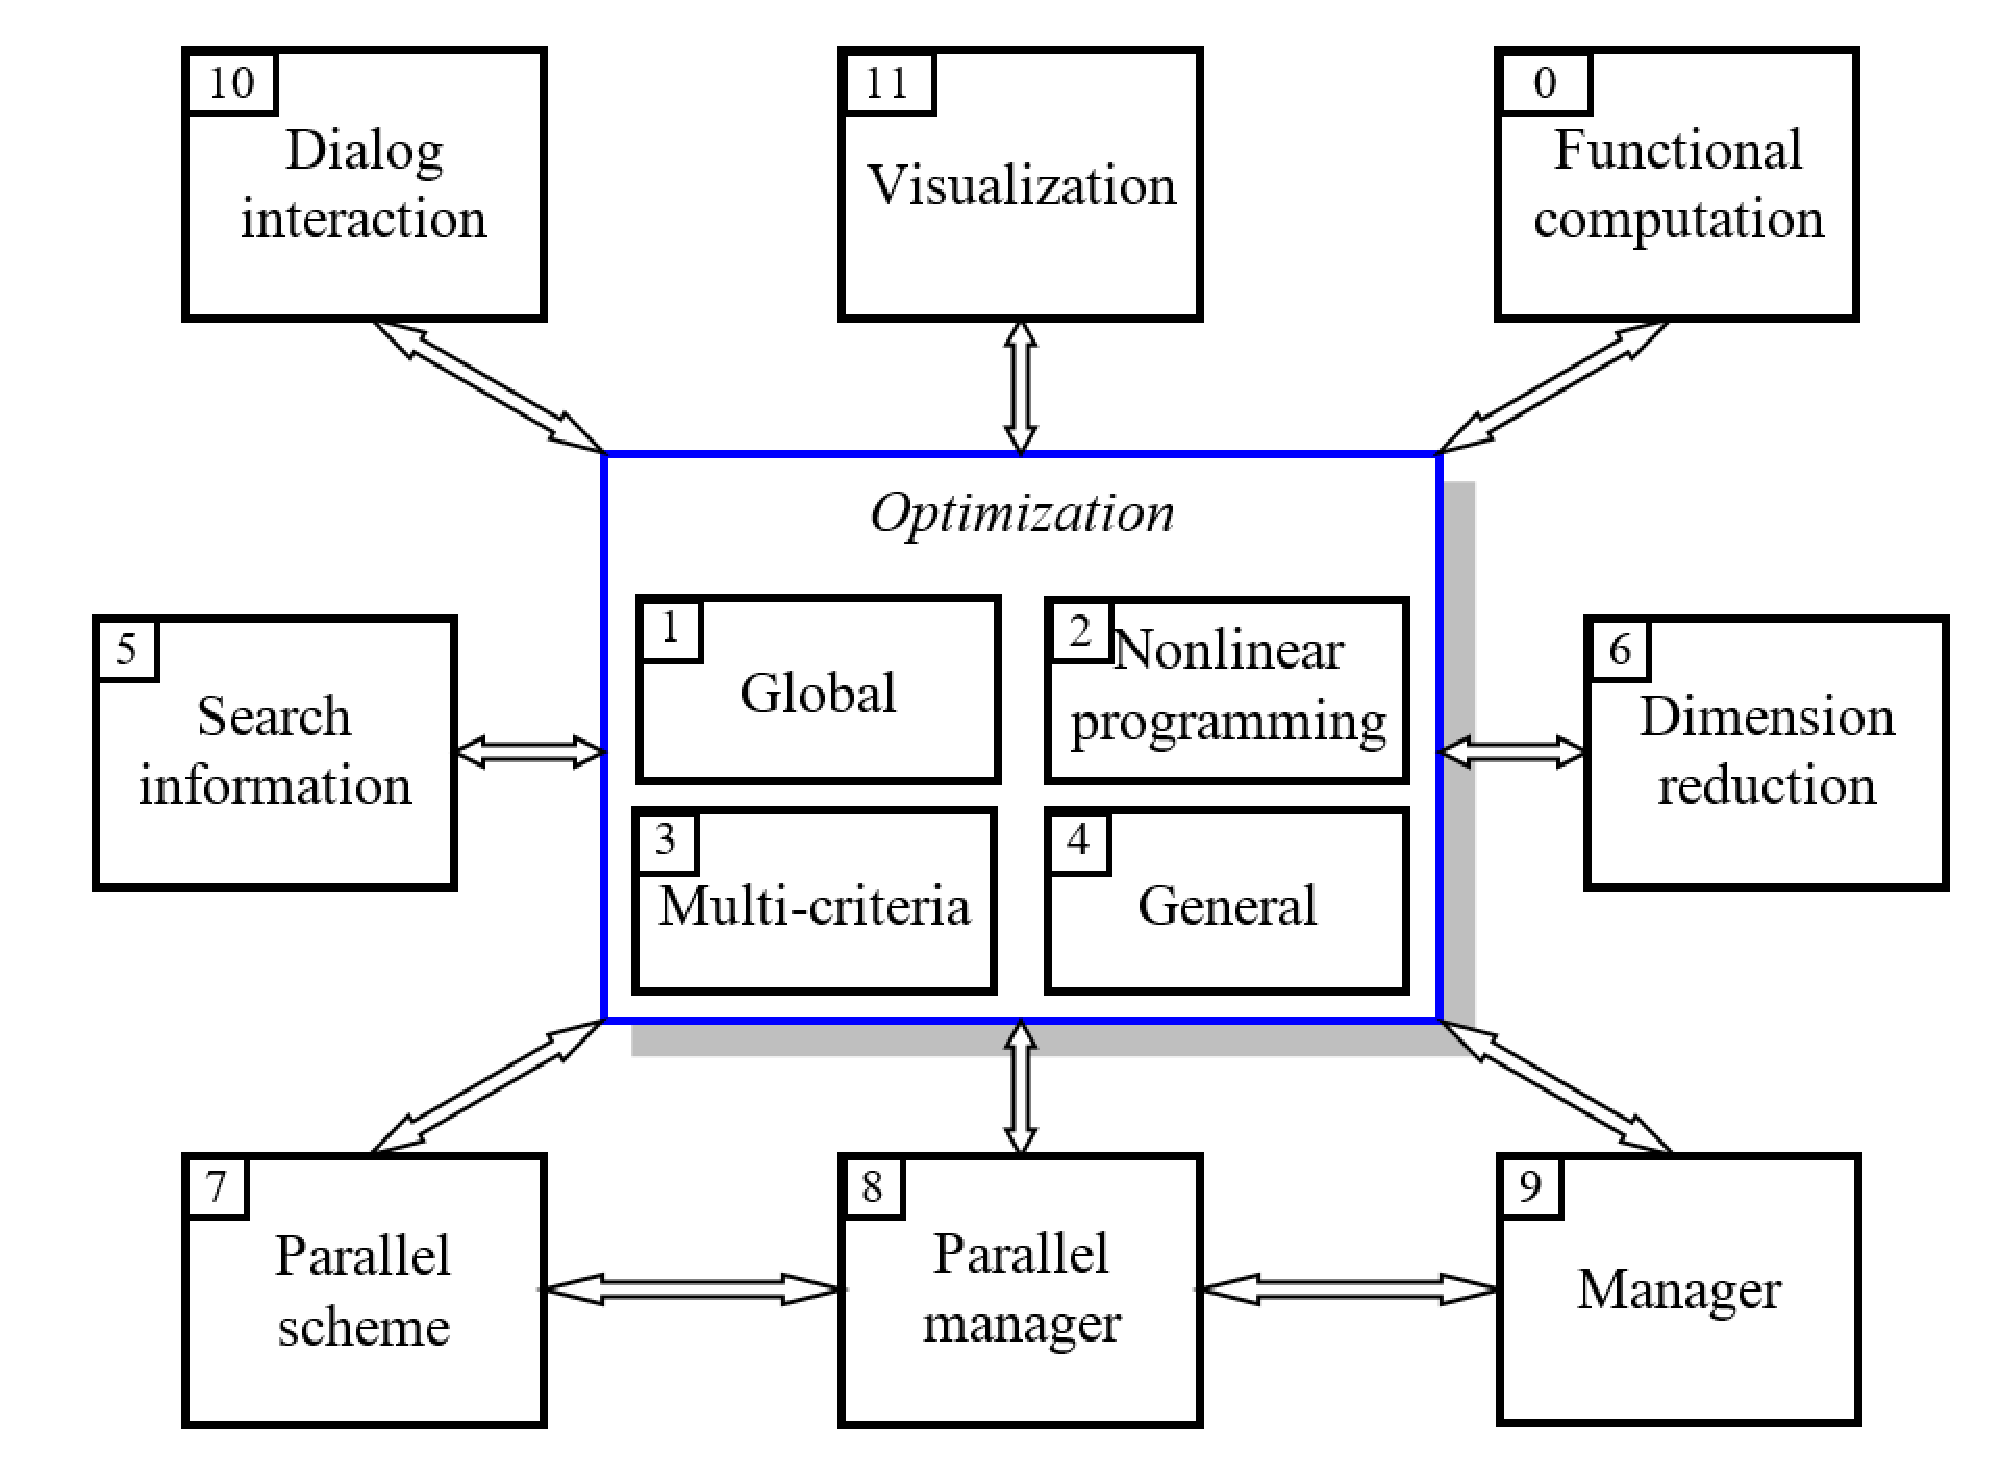
\includegraphics[width=0.75\textwidth]{pictures/globalizerScheme.eps}
    \caption{The Globalizer system architecture (Blocks 1-2, 5-7 have been implemented; Blocks 3-4 and 8-11 are under development)}
    \label{fig:globalizerScheme}
\end{figure}

\par
The Globalizer system architecture is presented in Figure \ref{fig:globalizerScheme}. The structural components are:
\begin{itemize}
  \item Block 0 consists of the procedures for computing the function values (criteria
  and constraints) for the optimization problem being solved; this is an external
  block with respect to the Globalizer system and is provided by the user per a predefined interface.
  \item Blocks 1-4 form the optimization subsystem and solve the global optimization
  problems (Block 1), nonlinear programming (Block 2), multicriterial optimization (Block 3),
  and general decision making problems (Block 4). It is worth noting the sequential
  scheme of interaction between these components --- the decision making problems are
  solved using the multicriterial optimization block, which, in turn, uses the nonlinear programming block, etc.
  \item Block 5 is a subsystem for accumulating and processing the search information;
  this is one of the basic subsystems --- the amount of search information for complex
  optimization problems may appear to be quite large on the one hand, but, on the other
  hand, the efficiency of the global optimization methods depends to a great extent on how
  completely all of the available search data is utilized.
  \item Block 6 contains the dimensional reduction procedures based on Peano evolvents;
  the optimization blocks solve the reduced (one-dimensional) optimization problems;
  Block 6 provides interaction between the optimization blocks and the initial
  multidimensional optimization problem.
  \item Block 7 organizes the choice of parallel computation schemes in the Globalizer
  system subject to the computing system architecture employed (the numbers of cores in the
  processors, the availability of shared and distributed memory, the availability of
  accelerators for computations, etc.) and the global optimization methods applied.
  \item Block 8 is responsible for managing the parallel processes when performing the
  global search (determining the optimal configuration of parallel processes, distributing
  the processes between computer elements, balancing computational loads, etc.).
  \item Block 9 is a common managing subsystem, which fully controls the whole
  computational process when solving global optimization problems.
  \item Block 10 is responsible for organizing the dialog interaction with users for
  stating the optimization problem, adjusting system parameters (if necessary), and
  visualizing and presenting the global search results.
  \item Block 11 is a set of tools for visualizing and presenting the global search results;
  the availability of tools for visually presenting the computational results enables
  the user to provide efficient control over the global optimization process.
\end{itemize}
\par
The Globalizer system comes in two different options:
\begin{itemize}
  \item Globalizer Pro is a research version of the system providing a full set of
  capabilities that are oriented toward solving of the most complicated global optimization problems.
  \item Globalizer Lite is a limited version of the Globalizer system accessible for free for
  solving global optimization problems with a medium level of difficulty, and is accessible free of charge.
\end{itemize}


\section{Results of Numerical Experiments}
\label{sec:experiments}
In order to confirm the operability of the Globalizer system, results from two
series of computational experiments are presented in this section.
\par
The computational experiments were conducted using the Lobachevsky supercomputer at the
State University of Nizhny Novgorod (operation system --- CentOS 6.4, management system --- SLURM).
Each supercomputer node had 2 Intel Sandy Bridge E5-2660 processors, 2.2 GHz, with 64 GB RAM.
Each processor had 8 cores (i.e. a total of 16 CPU cores were available at each node).
In order to generate the executable program code, the Intel C++ 14.0.2 compiler was used.
\par
A number of nodes in the computer system utilized Intel Xeon Phi 5110P processors,
each containing 60 cores (a total of 240 threads). In addition, the supercomputer also
included computer nodes equipped with two GPU NVIDIA Kepler K20X, each providing 14
stream multiprocessors (a total of 2688 CUDA-cores). In order to generate the executable
code, the CUDA Toolkit 6.0 was used.
\par
The problems generated by the GKLS-generator \cite{gavianoKvasovLeraSergeev2003}
were selected for the test problems. This generator allowed for obtaining the multiextremal
optimization problems with \textit{a priori} known properties: the number of local minima,
the sizes of their attractors, the global minimum point, the function value at this point, etc.
In order to simulate the computation costs inherent in the applied optimization problems (see, for example, \cite{Barkalov2013}, \cite{gergel2013}, \cite{gergel2015}), in all of the experiments computing the objective function was complicated by auxiliary computations, not altering the form of the function and the position of its minima.
\par
The computational experiments considered below were first carried out using the ExaMin system (see \cite{barkalovGergel2015}, \cite{barkalovGergelLebedev2015}, \cite{barkalovGergelLebedevSysoev2015}, \cite{gergelLebedev2015}) and then were reproduced using the Globalizer system.

\subsection{Comparison with over methods}

The results of numerical comparison of three sequential algorithms -- DIRECT \cite{Jones}, DIRECT\textit{l} \cite{Gablonsky} and core global search algorithm (GSA) from section \ref{subsec:corepar} -- are provided below (results of the work of the first two algorithms are given in paper \cite{gavianoKvasovLeraSergeev2003}). Numerical comparison was carried out on function classes \textit{Simple} and \textit{Hard} of dimension 4 and 5 from \cite{gavianoKvasovLeraSergeev2003} since solving a problems of dimension 2 and 3 demands a small number of iterations. Global minimizer $y^\ast$ was considered to be found, if the algorithm generated trial point $y^k$ in $\delta$-vicinity of the global minimum, i.e., $\left\|y^k-y^\ast\right\|\leq\delta$. The size of the vicinity was selected (according to \cite{gavianoKvasovLeraSergeev2003}) as $\delta = \left\|b-a\right\|\sqrt[N]{\Delta}$, $N$ -- problem dimension, $a$ and $b$ -- borders of search domain $D$, parameter $\Delta=10^{-6}$ at $N=4$ and $\Delta=10^{-7}$ at $N=5$. When using the GSA for the class \textit{Simple} parameter $r=4.5$ was selected, for the class \textit{Hard} $r=5.6$ was selected; evolvent construction parameter was fixed as $m=10$. The maximum allowable number of iterations was $K_{max} = 10^6$.

The average number of iterations $k_{av}$ performed by the method for solving a series of problems from these classes is shown in table \ref{tab:3}. Symbol ''$>$''  reflects a situation in which not all problems of the class were solved by the method. This means that the algorithm was stopped as the maximum allowable number of iterations $K_{max}$ was achieved. In this case, value $K_{max}=10^6$ was used for calculating the average value of the number of iterations $k_{av}$ that corresponds to the lower estimate of this average value. The number of unsolved problems is specified in brackets.

\begin{table}
  \caption{Average number of iterations $k_{av}$}
  \label{tab:3}
  \center
  \begin{tabular}{lllll}
    \hline\noalign{\smallskip}
     $N$ & Problem class & DIRECT & DIRECT\textit{l} & GSA \\
    \noalign{\smallskip} \hline \noalign{\smallskip}
      4 &	\textit{Simple}	& $>$47282(4) &	18983 &	11953 \\
        & \textit{Hard} &	$>$95708(7) &	68754 &	25263 \\
      5	& \textit{Simple} &	$>$16057(1) &	16758 &	15920 \\
        & \textit{Hard} &	$>$217215(16) &	$>$269064(4) & $>$148342(4) \\
    \noalign{\smallskip}\hline
  \end{tabular}
\end{table}

Table \ref{tab:3} shows that GSA outperforms DIRECT and DIRECT\textit{l} methods on all classes of problems in terms of average number of iterations. In class 5-\textit{Hard} all three methods failed to solve all problems: DIRECT did not solve 16 problems, DIRECT\textit{l} and GSA, 4 problems.


\subsection{Parallel Computations Using Intel Xeon Phi processors}
The results of the numerical experiments with GPMAGS on an Intel Xeon Phi are provided in Table \ref{tab:exResults}.
The computations were performed using the \textit{Simple} and \textit{Hard} function classes with the
dimensions equal to 4 and 5. The parameters \(\Delta=10^{-6}\) at \(N=4\) and \(\Delta=10^{-6}\) at \(N=5\)
were used. When using the GPMAGS method, the parameter \(r=4.5\) was selected for the
\textit{Simple} class, and \(r=5.6\) was selected for the \textit{Hard} class.
\par
In the first series of experiments, serial computations using MAGS were executed.
The average number of iterations performed by the method for solving a series of
problems for each of these classes is shown in row I. The symbol ``\(>\)'' reflects the
situation where not all problems of a given class were solved by a given method.
It means that the algorithm was stopped once the maximum allowable number of
iterations \(K_{max}\) was achieved. In this case, the \(K_{max}\) value was used for
calculating the average number of iterations corresponding to the lower estimate of
this average value. The number of unsolved problems is specified in brackets.
\par
In the second series of experiments, parallel computations were executed on a CPU.
The relative ``speedup'' in iterations achieved is shown in row II; the speedup of
parallel computations was measured in relation to the sequential computations (\(p=1\)).

\begin{table}
  \centering
  \label{tab:exResults}
  \caption{Results of numerical experiments}
  \begin{tabular}{cccccccc}
    \cline{3-8}\noalign{\smallskip}
    \multicolumn{2}{c}{  } & \textit{p} & \multicolumn{2}{c}{$N=4$} & & \multicolumn{2}{c}{$N=5$}   \\
    \noalign{\smallskip} \cline{4-5} \cline{7-8}  \noalign{\smallskip}
    \multicolumn{2}{c}{  } & & \textit{Simple} & \textit{Hard} & & \textit{Simple} & \textit{Hard}  \\
    \noalign{\smallskip}\hline
    I &
    \parbox{0.25\textwidth}{
    \begin{center}
    \textbf{Serial computations.}\\ \textit{Average number} \\ \textit{of iterations.}
    \end{center}		}
      & 1 & 11953 & 25263 & & 15920 & \(>\)148342 (4)  \\
    \hline \noalign{\smallskip}
II  & \textbf{Parallel computations}  %\multirow{3}{*}{}
  & 2 & 2.51 & 2.26 & & 1.19 & 1.36 \\
& \textbf{of CPU}. & 4 & 5.04 & 4.23 & & 3.06 & 2.86 \\
& \textit{Speedup} & 8 & 8.58 & 8.79 & & 4.22 & 6.56 \\
    \noalign{\smallskip}\hline	\noalign{\smallskip}
III & \textbf{Parallel computations} %\multirow{3}{*}{}
  & 60  & 8.13 & 7.32 & & 9.87 & 6.55  \\
&  o\textbf{f Xeon Phi}. & 120 & 16.33 & 15.82 & & 15.15 & 17.31 \\
& \textit{Speedup} & 240 & 33.07 & 27.79 & & 38.80 & 59.31 \\

    \noalign{\smallskip}\hline
  \end{tabular}
\end{table}

\par
The final series of experiments was executed using a Xeon Phi. The results of these
computations are shown in row III; in this case, the speedup factor is calculated in
relation to the PMAGS results on a CPU using eight cores (\(p=8\)). It can be noted that
relatively high speedup was achieved. For example, solving a problem from the 5-\textit{Hard} class
required on average only 633 parallel iterations on the Xeon Phi, whereas the number of
iterations was more than 37 thousand when using all of the CPU’s computing cores.

\subsection{Parallel Computations Using General Purpose Graphic Processors}
In the first series of experiments, only one graphic accelerator was used for solving
100 6-diminsional problems. The method’s reliability parameter \(r=4.5\) was selected.
\par
The average problem solving time using a GPU was 10.78 sec. whereas the averaged problem
solving time using all of the node’s 16 CPU cores was 53.8 sec.; an almost 5-fold improvement was observed.
\par
A larger scale computational experiment was carried out for the problems with
dimensions of \(N=8\) and \(N=10\): a total of 12 nodes within a cluster with 36
graphic accelerators (three accelerators per node) were employed, therefore, a total
of 96768 CUDA-cores were employed.
\par
The average time to solve the 8-dimensional problem was 405.6 seconds, 5.9 times
faster than the CPU version of the algorithm. The average time to solve the
10-dimensional problem was 2,055.8 sec. The CPU was not used to solve the 10-dimensional
problem because of the high degree of complexity in the computations.

\section{Conclusions} \label{sec:concl}

In this paper, the Globalizer global optimization system for solving the time-consuming global optimization problems using a wide spectrum of high-performance computational systems (the systems with shared and distributed memory, the systems with NVIDIA graphic processors and Intel Xeon Phi coprocessors) was considered. The highly parallel computations were facilitated using various distinctive computational schemes: processing several optimization iterations simultaneously, reducing multidimensional optimization problems using multiple Peano space-filling curves, and the multi-stage computing based on nested block reduction schemes. The numerical experiments have confirmed the efficiency of the Globalizer system.

In future, it is planned to extend the Globalizer system for solving the multicriterial multiextremal multidimensional optimization problems with the nonlinear constraints. As a valuable part of further work, Globalizer would be used for solving the applied optimization problems from various application fields.
% You may incorporate your references as follows in your main tex file.
% Using BibTex is not recommended but can be handled.
%\bibliographystyle{plain}
%\bibliography{paper}

\begin{thebibliography}{10}

\bibitem{barkalovGergel2014}
\newblock K. A. Barkalov and V. P. Gergel,
\newblock Multilevel scheme of dimensionality reduction for parallel global search algorithms,
\newblock in \emph{Proceedings of the 1st International Conference on
  Engineering and Applied Sciences Optimization}, (2014), 2111--2124.

\bibitem{barkalovGergel2015}[10.1007/s10898-016-0411-y]
\newblock K. Barkalov and V. Gergel,
\newblock Parallel global optimization on GPU,
\newblock \emph{J. Glob. Optim.}, \textbf{66(1)} (2016), 3--20.

\bibitem{barkalovGergelLebedev2015}[10.1007/978-3-319-21909-7_31]
\newblock K. Barkalov, V. Gergel and I. Lebedev,
\newblock Use of XeonPhi coprocessor for solving global optimization problems,
\newblock \emph{LNCS}, \textbf{9251} (2015), 307--318.

\bibitem{barkalovGergelLebedevSysoev2015}
\newblock K. Barkalov, V. Gergel, I. Lebedev, A. Sysoev, %http://ceur-ws.org/Vol-1482/
\newblock Solving the global optimization problems on heterogeneous cluster systems,
\newblock in \emph{CEUR Workshop Proceedings}, \textbf{1482} (2015), 411--419.
%\newblock (In Russian).

\bibitem{Barkalov2013}[10.1007/978-3-642-39958-9_14]
\newblock K. Barkalov, A. Polov inkin, I. Meyerov, S. Sidorov, N. Zolotykh,
\newblock SVM regression parameters optimization using parallel global search algorithm,
\newblock \emph{LNCS}, \textbf{7979} (2013), 154--166.

\bibitem{bussieckMeeraus2004}[10.1007/978-1-4613-0215-5_8]
\newblock M. R. Bussieck and A. Meeraus,
\newblock General algebraic modeling system (GAMS), in \emph{Modeling Languages in Mathematical Optimization} (ed. J. Kallrath),
\newblock Springer (2004), 137--157.

\bibitem{censorZeniosParGO}
\newblock Y. Censor and S. A. Zenios,
\newblock \emph{Parallel optimization: theory, algorithms, and applications},
\newblock Oxford University Press (1998).

\bibitem{ciegisHentyParGO}[10.1007/978-0-387-09707-7]
\newblock R. Ciegis, D. Henty, B. Kågström and J. Zilinskas,
\newblock \emph{Parallel scientific computing and optimization: advances and applications},
\newblock Springer (2009).

\bibitem{iosoDescription}
\newblock I. N. Egorov, G. V. Kretinin, I. A. Leshchenko and S. V. Kuptzov,
\newblock IOSO optimization toolkit --- novel software to create better design,
\newblock in \emph{9th AIAA/ISSMO Symposium on Multidisciplinary Analysis and Optimization}, 2002.
\newblock Available from \url{http://www.iosotech.com/text/2002\_4329.pdf}.

\bibitem{Famularo1999}[10.1016/S0005-1098(99)00058-8]
\newblock D. Famularo and P. Pugliese and Ya. D. Sergeyev,
\newblock A global optimization technique for checking parametric robustness,
\newblock \emph{Automatica}, \textbf{35} (1999), 1605--1611.

\bibitem{fasanoPinter2013}[10.1007/978-1-4614-4469-5]
\newblock G. Fasano and J. D. Pinter,
\newblock \emph{Modeling and optimization in space engineering},
\newblock Springer, 2013.

\bibitem{floudasPardalosGOState}[10.1007/978-1-4613-3437-8]
\newblock C. A. Floudas and M. P. Pardalos,
\newblock \emph{State of the art in global optimization: computational methods and applications},
\newblock Kluwer Academic Publishers, Dordrecht (1996).

\bibitem{floudasPardGO}[10.1007/s10898-008-9332-8]
\newblock C. A. Floudas and M. P. Pardalos,
\newblock \emph{Recent advances in global optimization},
\newblock Princeton University Press (2016).

\bibitem{Gablonsky}[10.1023/A:1017930332101]
\newblock J. M. Gablonsky and C. T. Kelley,
\newblock A locally-biased form of the DIRECT algorithm,
\newblock \emph{J. Glob. Optim.}, \textbf{21(1)} (2001), 27--37.

\bibitem{gavianoKvasovLeraSergeev2003}[10.1145/962437.962444]
\newblock M. Gaviano and D.E. Kvasov and D. Lera and Ya.D. Sergeev,
\newblock Software for generation of classes of test functions with known local and global minima for global optimization,
\newblock \emph{ACM Trans. Math. Software}, \textbf{29(4)} (2003), 469--480.

\bibitem{gergelLebedev2015}[10.1016/j.procs.2015.11.008]
\newblock V. Gergel and I. Lebedev,
\newblock Heterogeneous parallel computations for solving global optimization problems,
\newblock \emph{Procedia Comput. Sci.}, \textbf{66} (2015), 53--62.

\bibitem{gergel1993}
\newblock V. P. Gergel,
\newblock A software system for multi-extremal optimization,
\newblock \emph{Eur. J. Oper. Res.}, \textbf{65(3)} (1993), 305--313.

\bibitem{gergel1996}
\newblock V. P. Gergel,
\newblock A method for using derivatives in the minimization of multiextremum functions,
\newblock \emph{Comput. Math. Math. Phys.}, \textbf{36(6)} (1996), 729--742.

\bibitem{gergel1997}[10.1023/A:1008290629896]
\newblock V. P. Gergel,
\newblock A global optimization algorithm for multivariate functions with lipschitzian first derivatives,
\newblock \emph{J. Glob. Optim.}, \textbf{10(3)} (1997), 257--281.

\bibitem{gergel2013}[doi:10.1016/j.procs.2013.05.164]
\newblock V. P. Gergel, et al.,
\newblock High performance computing in biomedical applications,
\newblock \emph{Procedia Computer Science}, \textbf{18} (2013), 10--19.

\bibitem{gergel2015}[10.15866/ireaco.v8i1.4935]
\newblock V. P. Gergel, et al.,
\newblock Recognition of surface defects of cold-rolling sheets based on method of localities,
\newblock \emph{International Review of Automatic Control }, \textbf{8(1)} (2015), 51--55.

\bibitem{gergelSidorov2015}[10.1007/978-3-319-21909-7_49]
\newblock V. P. Gergel and S. V. Sidorov,
\newblock A two-level parallel global search algorithm for solving computationally intensive multi-extremal optimization problems,
\newblock \emph{LNCS}, \textbf{9251} (2015), 505--515.

\bibitem{grishaginStrongin1984}
\newblock V. A. Grishagin and R. G. Strongin,
\newblock Optimization of multi-extremal functions subject to monotonically unimodal constraints,
\newblock \emph{Engineering Cybernetics}, \textbf{5} (1984), 117--122.

\bibitem{holmstromEdvall2004}[10.1007/978-1-4613-0215-5_19]
\newblock K. Holmström and M. M. Edvall,
\newblock The TOMLAB optimization environment,
\newblock \emph{Modeling Languages in Mathematical Optimization},
\newblock 369--376, Springer (2004).

\bibitem{horstTuyGO}[10.1007/978-3-662-03199-5]
\newblock R. Horst and H. Tuy,
\newblock \emph{Global optimization: deterministic approaches},
\newblock Springer-Verlag, Berlin (1990).

\bibitem{Jones}[10.1007/BF00941892]
\newblock D. R. Jones, C. D. Perttunen and B. E. Stuckman,
\newblock Lipschitzian optimization without the Lipschitz constant,
\newblock \emph{J. Optim. Theory Appl.}, \textbf{79(1)} (1993), 157--181.

\bibitem{kearfott2009}[10.1080/10556780802614051]
\newblock R. B. Kearfott,
\newblock GlobSol user guide,
\newblock \emph{Optim. Methods Softw.}, \textbf{24} (2009), 687--708.

\bibitem{Kvasov2015}[10.1016/j.advengsoft.2014.09.014]
\newblock D. E. Kvasov and Ya. D. Sergeyev,
\newblock Deterministic approaches for solving practical black-box global optimization problems,
\newblock \emph{Adv. Eng. Softw.}, \textbf{80} (2015), 58--66.

\bibitem{Menniti}[10.1016/j.epsr.2007.10.009]
\newblock D. E. Kvasov, D. Menniti, A. Pinnarelli, Ya. D. Sergeyev and N. Sorrentino,
\newblock Tuning fuzzy power-system stabilizers in multi-machine systems by global optimization algorithms based on efficient domain partitions,
\newblock \emph{Electric Power Systems Research}, \textbf{78(7)} (2008), 1217--1229.

\bibitem{Pizzuti}[10.1007/s00211-002-0419-8]
\newblock D. E. Kvasov, C. Pizzuti and Ya. D. Sergeyev,
\newblock Local tuning and partition strategies for diagonal go methods,
\newblock \emph{Numerische Mathematik}, \textbf{94(1)} (2003), 93--106.

\bibitem{liberti2009}[10.1007/0-387-30528-9_8]
\newblock L. Liberti,
\newblock Writing global optimization software,
\newblock in \emph{Nonconvex Optimization and Its Applications }, \textbf{84}, 211--262,
\newblock Springer (2006).

\bibitem{linSchrage2009}[10.1080/10556780902753221]
\newblock Y. Lin and L. Schrage,
\newblock The global solver in the LINDO API,
\newblock \emph{Optim. Methods Softw.}, \textbf{24(4-5)} (2009), 657--668.

\bibitem{locatelliSchoenGO}[10.1137/1.9781611972672]
\newblock M. Locatelli and F. Schoen,
\newblock \emph{Global optimization: theory, algorithms and applications},
\newblock SIAM (2013).

\bibitem{luqueAlbaGA}[10.1007/978-3-642-22084-5]
\newblock G. Luque and E. Alba,
\newblock \emph{Parallel genetic algorithms. Theory and real world applications},
\newblock Springer-Verlag, Berlin (2011).

\bibitem{mongeauKarsentyRouze2000}[10.1080/10556780008805783]
\newblock M. Mongeau, H. Karsenty, V. Rouzé and J. B. Hiriart-Urruty,
\newblock Comparison of public-domain software for black box global optimization,
\newblock \emph{Optim. Methods Softw.}, \textbf{13} (2000), 203--226.

\bibitem{mullen2014}[10.18637/jss.v060.i06]
\newblock K. M. Mullen,
\newblock Continuous global optimization in R,
\newblock \emph{J. Stat. Softw.}, \textbf{60(6)} (2014).

\bibitem{pardalosZhigljavskyZilinskas2016}[10.1007/978-3-319-29975-4]
\newblock M. P. Pardalos, A. A. Zhigljavsky and J. Zilinskas,
\newblock \emph{Advances in stochastic and deterministic global optimization},
\newblock Springer (2016).

\bibitem{pinterGO}[10.1007/978-1-4757-2502-5]
\newblock J. D. Pinter,
\newblock \emph{Global optimization in action (Continuous and Lipschitz optimization: algorithms, implementations and applications)},
\newblock Kluwer Academic Publishers, Dordrecht (1996).

\bibitem{pinter2009}
\newblock J. D. Pinter,
\newblock Software development for global optimization,
\newblock \emph{Lectures on Global Optimization. Fields Institute Communications}, \textbf{55} (2009), 183--204.

\bibitem{riosSahinidis2013}[10.1007/s10898-012-9951-y]
\newblock L. M. Rios and N. V. Sahinidis,
\newblock Derivative-free optimization: a review of algorithms and comparison of software implementations,
\newblock \emph{J. Glob. Optim.}, \textbf{56} (2013), 1247--1293.

\bibitem{sahinidis1996}[10.1007/BF00138693]
\newblock N. V. Sahinidis,
\newblock BARON: A general purpose global optimization software package,
\newblock \emph{J. Glob. Optim.}, \textbf{8} (1996), 201--205.

\bibitem{sergeyev1995}[10.1137/0805041]
\newblock Y. D. Sergeyev,
\newblock An information global optimization algorithm with local tuning,
\newblock \emph{SIAM J. Optim.}, \textbf{5(4)} (1995), 858--870.

\bibitem{sergeyev1999}
\newblock Y. D. Sergeyev,
\newblock Multidimensional global optimization using the first derivatives,
\newblock \emph{Comput. Math. Math. Phys.}, \textbf{39(5)} (1999), 743--752,.

\bibitem{sergeyevGrishagin1994}[10.1007/BF02207778]
\newblock Y. D. Sergeyev and V. A. Grishagin,
\newblock A parallel method for finding the global minimum of univariate functions,
\newblock \emph{Journal of Optimization Theory and Applications}, \textbf{80(3)} (1994), 513--536.

\bibitem{sergeyevGrishagin2001}[10.1023/A:1010185125012]
\newblock Y. D. Sergeyev and V. A. Grishagin,
\newblock Parallel asynchronous global search and the nested optimization scheme,
\newblock \emph{J. Comput. Anal. Appl.}, \textbf{3(2)} (2001), 123--145.

\bibitem{sergeyevStronginLera2013}[10.1007/978-1-4614-8042-6]
\newblock Y. D. Sergeyev, R. G. Strongin and D. Lera,
\newblock \emph{Introduction to global optimization exploiting space-filling curves},
\newblock Springer (2013).

\bibitem{Famularo2001}[10.1023/A:1012391611462]
\newblock Ya. D. Sergeyev, D. Famularo and P. Pugliese,
\newblock Index branch-and-bound algorithm for lipschitz univariate global optimization with multiextremal constraints,
\newblock \emph{J. Glob. Optim.}, \textbf{21(3)} (2001), 317--341.

\bibitem{strongin1978}
\newblock R. G. Strongin,
\newblock \emph{Numerical methods in multi-extremal problems (information-statistical algorithms)},
\newblock Moscow: Nauka, In Russian (1978).

\bibitem{strongin1992}[10.1007/BF00122428]
\newblock R. G. Strongin,
\newblock Algorithms for multi-extremal mathematical programming problems employing a set of joint space-filling curves,
\newblock \emph{J. Glob. Optim.}, \textbf{2(4)} (1992), 357--378.

\bibitem{stronginGergelBarkalovParGO}
\newblock R. G. Strongin, V. P. Gergel, V. A. Grishagin and K. A. Barkalov,
\newblock \emph{Parallel computations for global optimization problems},
\newblock Moscow State University (In Russian), Moscow (2013).

\bibitem{strSergGO}[10.1007/978-1-4615-4677-1]
\newblock R.G. Strongin and Ya.D. Sergeyev,
\newblock \emph{Global optimization with non-convex constraints. Sequential and parallel algorithms},
\newblock Kluwer Academic Publishers, Dordrecht (2000).

\bibitem{zilinskTornGO}[10.1007/3-540-50871-6]
\newblock A. Törn and A. Zilinskas,
\newblock \emph{Global optimization},
\newblock Springer (1989).

\bibitem{venkataraman2009}
\newblock P. Venkataraman,
\newblock \emph{Applied optimization with MATLAB programming},
\newblock John Wiley \& Sons (2009).

\bibitem{zhigljavskyRandGO}[10.1007/978-94-011-3436-1]
\newblock A. A. Zhigljavsky,
\newblock \emph{Theory of global random search},
\newblock Kluwer Academic Publishers, Dordrecht (1991).

\end{thebibliography}

\medskip
% The data information below will be filled by AIMS editorial staff
Received xxxx 20xx; revised xxxx 20xx.
\medskip

\end{document}
